\documentclass[conference]{IEEEtran}
\usepackage{caption}
\IEEEoverridecommandlockouts
% The preceding line is only needed to identify funding in the first footnote. If that is unneeded, please comment it out.
\usepackage{cite}
\usepackage{amsmath,amssymb,amsfonts}
\usepackage{algorithmic}
\usepackage{graphicx}

% for multiple image adding
\usepackage{caption}
\usepackage{graphicx}
\usepackage{subcaption}



\hyphenation{op-tical net-works semi-conduc-tor}



\begin{document}

% \title{Toward a Multi-Agent Approach for Dynamic Traffic Control and Optimization}

\title{Toward a Multi Agent Approach for LLM-Based Dynamic Vehicle Control and Communication in Accidental Condition}

% author names and affiliations
% use a multiple column layout for up to three different
% affiliations
\author{\IEEEauthorblockN{Rafi Md Ashifujjman}
\IEEEauthorblockA{\textit{Graduate School of}\\
\textit{Integrated Science and Technology}\\
\textit{Shizuoka University}\\Hamamatsu, Japan\\ ashifujjman@gmail.com}
\and

\IEEEauthorblockN{Naoki Fukuta}
\IEEEauthorblockA{\textit{College of Informatics, Academic Institute}\\
\textit{Shizuoka University}
\\Hamamatsu, Japan\\fukuta@inf.shizuoka.ac.jp}}

\maketitle
%done with tittle means name , author , etc.

% in the abstract
\begin{abstract}

\end{abstract}


\IEEEpeerreviewmaketitle



\section{Introduction}

This paper explores the potential of integrating Large Language Models (LLMs)\cite{zhang2024instruct} into a multi-agent framework to improve decision making in autonomous vehicles (AVs), particularly in unknown and unsafe domains.
Our main concern would be \textbf{ to explore the use of large language models (LLM) for autonomous driving systems(ADS) as the main decision-making agent within a multi-agent framework to evaluate its reasoning ability to handle long-tail, False positive, and False negative scenarios.} Our goal is to contribute to the development of safer and more reliable Level 5\cite{balasubramaniam2022object} autonomous vehicles. We aim to contribute for level 5 (complete automation \cite{raza2018autonomous}). There are numerous instances in which traditional autonomous vehicles are capable of making effective decisions in familiar scenarios using pre-trained models.  However, they may have trouble facing new or unusual situations where their programmed knowledge is not directly covered in such situations. Human drivers can use common sense and past experiences to handle unexpected events, such as knowing that traffic cones on a moving truck are not dangerous. However, current AV systems, even those that use rule-based approaches or reinforcement learning (RL\cite{kaelbling1996reinforcement}), will struggle in these scenarios. This limitation is especially evident in what we call "unknown-unsafe" region situations where the correct action is not immediately clear \cite{fu2024drive}.
During this investigation with various LLM, we proceed our investigation under two assumptions: 1) certain AIs can transform real-world situations into text-based explanations, which are subsequently used as input for the LLMs, and 2) the outputs generated by the LLMs can be translated into actual decisions made by the decision agent of AV by interpreting the responses from the LLMs. We are investigating the effectiveness of various Large Language Models (LLMs) for use as decision-making agents in autonomous driving systems. Our initial objective is to answer the research question, \textbf{Can an agent make decisions with the help of an LLM without undergoing a specific learning process for each new situation?}
In our research, we will assume that vehicle-to-vehicle (V2V) communication has been achieved through a standardized networking protocol, such as LAN-based direct communication or a low-latency wireless system. Under this assumption, each vehicle can communicate with other vehicles within a defined radius (e.g., 10 meters). When a vehicle enters the information sharing radius of another vehicle, they exchange data regarding their current status, such as obstacle detection, traffic conditions, speed, direction, and future intended actions.
To evaluate the impact of V2V communication on autonomous decision-making, we will investigate how Large Language Models (LLMs) process and utilize this information. Specifically, we will examine whether the incorporation of V2V exchanged data improves decision accuracy and enables AVs to make more precise and context-aware decisions.
However, V2V communication introduces a critical question,\textbf{ Is a single centralized decision-making agent sufficient to process all incoming V2V data and make autonomous driving decisions, or is a multi-agent system required for improved efficiency and scalability?}



\section{Motivation and Background}
\begin{figure}[ht]
    \centering
    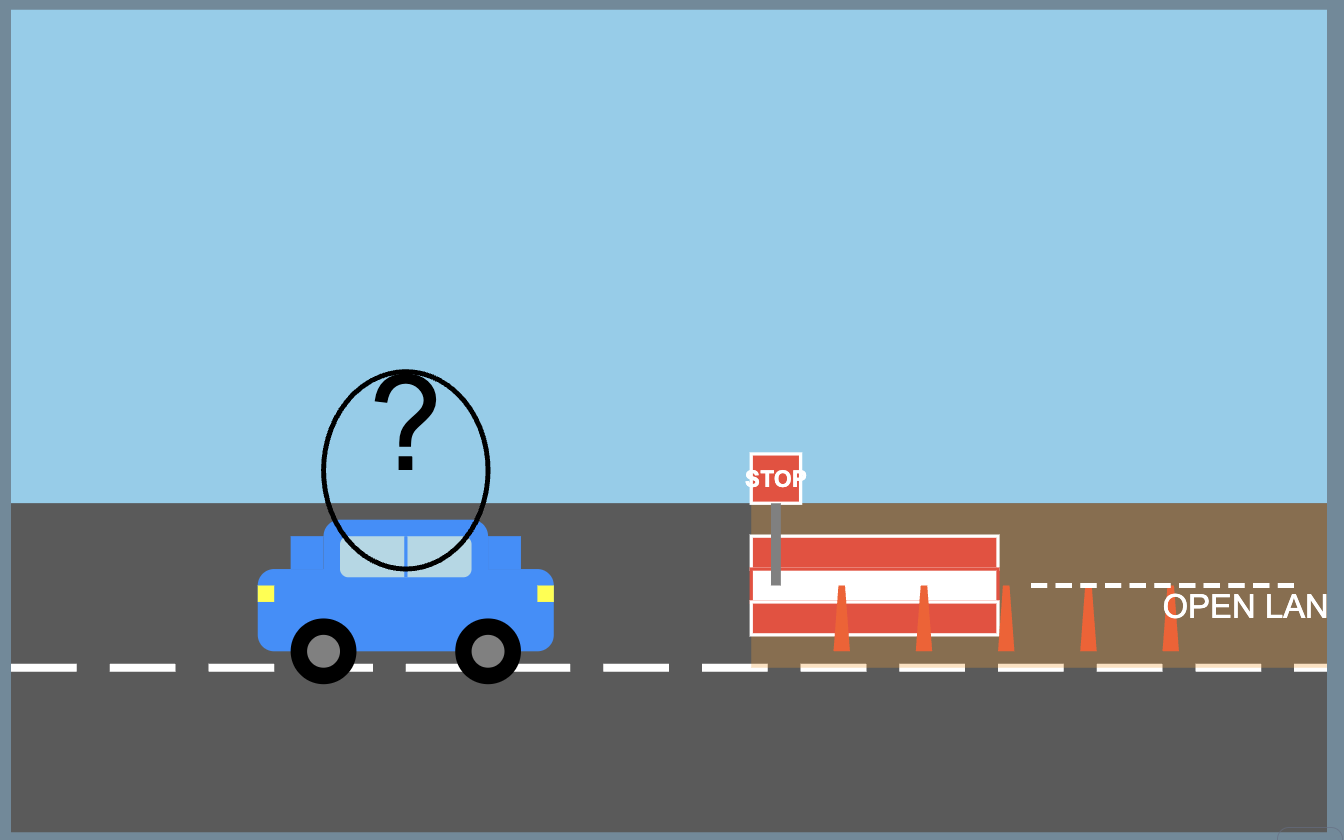
\includegraphics[width= \linewidth]{situation1.png}
    \caption{What current AV might do in this situation?}
    \label{fig:enter-label-unique}
\end{figure}
Imagine a situation where a road is partially blocked due to construction, with traffic cones and a "STOP" sign indicating obstruction. A typical autonomous vehicle (AV) might see the "STOP" sign and interpret it as a complete road closure, coming to a complete stop because that is what its pre-programmed data tell it to do. However, a human driver in the same situation might use common sense, realize that the road is only partially closed, and safely continue through the open section.
\begin{figure}[ht]
    \centering
    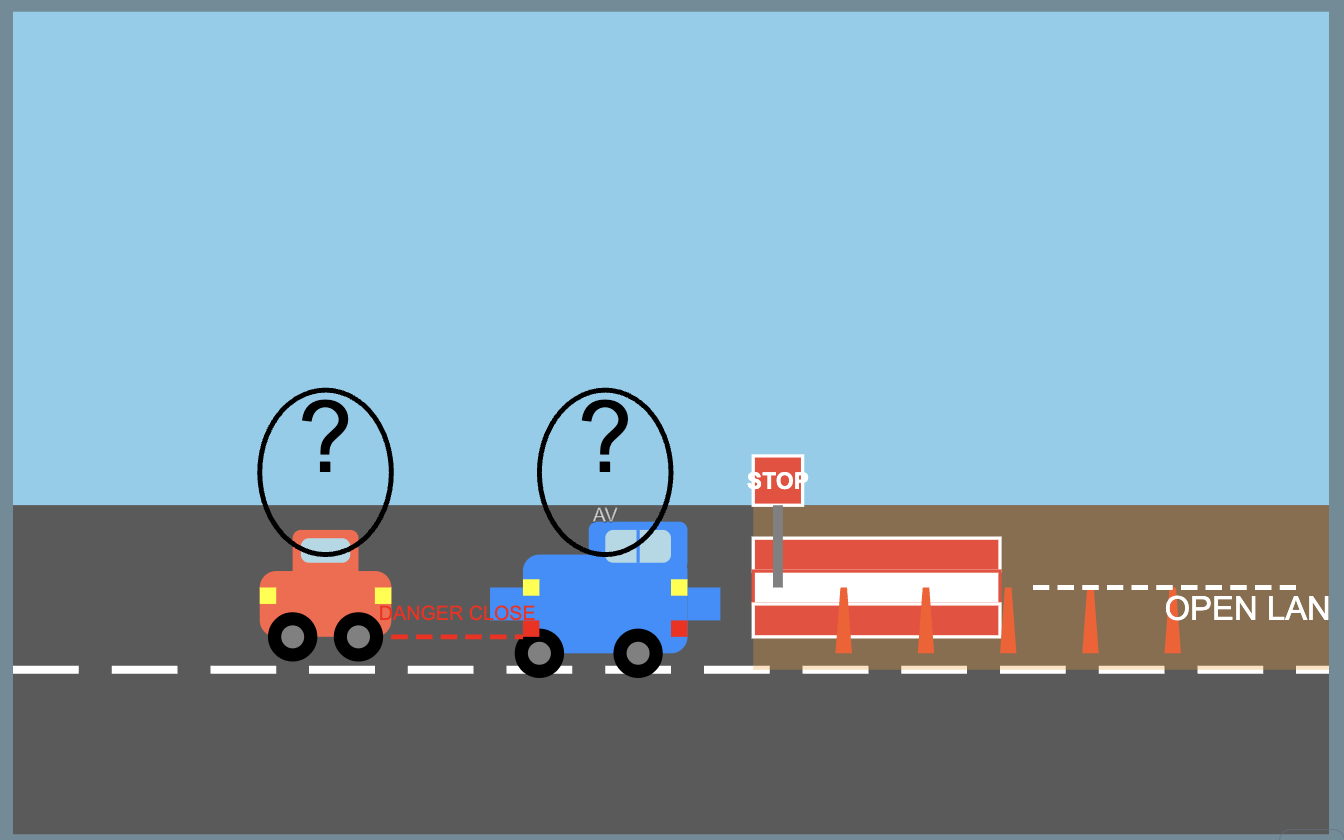
\includegraphics[width= \linewidth]{situation2.png}
    \caption{Lack of communication between vehicles may lead to a potential accident.}
    \label{fig:enter-label-unique-2}
\end{figure}

Now, let us make it more complicated that an autonomous truck comes to a sudden stop when it sees the "STOP" sign. There is another car, driven by a human or another AV, right behind it. This sudden stop could easily cause a crash. 
Now imagine a human driver encountering a partially blocked road. To navigate safely, the driver shifts into the adjacent open lane, relying on instinct and situational awareness. Anticipating the possibility of an oncoming vehicle from the opposite direction or from behind, the driver proactively slows down, assessing the risk and taking the necessary precautions to avoid a collision. In contrast, a traditional AV, which lacks human-like reasoning and predictive thinking, may not recognize the potential danger. Without contextual understanding, it can continue at its normal speed, assuming the lane is clear, increasing the risk of a head-on collision.

However, if the AV had better reasoning abilities, it might recognize that the road is only partially closed and proceed safely through the open part. And if the AV could communicate with the vehicle behind it or if the lane was suddenly closed, it could alert the other car about its actions, preventing a possible accident.
A fundamental challenge in traditional autonomous vehicles (AVs) is to prepare for all truly unknown situations\cite{singh2024systematic}. Any scenario we create is technically "known" to us, even if it feels unfamiliar to the AV, making it difficult to test how AVs handle truly unknown-unsafe situations. In addition, it is difficult to recreate complex real-world scenarios in simulation environments. For example, it is difficult to accurately simulate unpredictable human actions or complicated environmental conditions. In real life, there are countless rare or unexpected situations that are nearly impossible to include in training data sets for traditional autonomous driving systems (ADS). Human drivers use common sense to deal with these situations, so we need to explore whether LLMs can also show human-like reasoning to handle them effectively. To address these challenges, we propose a possible approach on integrating Large Language Models (LLMs) into a multi-agent framework for autonomous driving control system. LLMs have the potential to provide common sense or reasoning ability that traditional systems lack, helping AVs better understand the context of complex real-world scenarios. Incorporating Vehicle-to-Vehicle communication using multi-agent, which allows vehicles to exchange information with other vehicles. This capability is also essential for creating realistic and complex driving scenarios.

\section{Preliminary}
Reasoning is a fundamental aspect of human intelligence, essential for problem solving, decision-making, and critical thinking. In recent years, Large Language Models (LLMs) have demonstrated emergent abilities\cite{wei2022emergent}, such as in-context learning\cite{dong2022survey}, role play\cite{shanahan2023role} and analogical reasoning\cite{wei2022chain}. These abilities allow LLMs to go beyond natural language processing problems to facilitate a wider range of tasks, such as code generation\cite{gehring2024rlef}, robotic control\cite{ahn2022can}, and autonomous agents\cite{deng2023mind2web}. Among these abilities, human-like reasoning has garnered significant attention from both academia and industry, since it demonstrates great potential for LLMs to generalize to complex real-world problems through abstract and logical reasoning. A notable breakthrough in this area is the 'chain of thought' prompting technique\cite{wei2022chain}, which can elicit step-by-step human-like reasoning processes at test time without any additional training. 

\section{Our Approach}








\section{Conclusion}
 
\begin{figure}[ht]
    \centering
    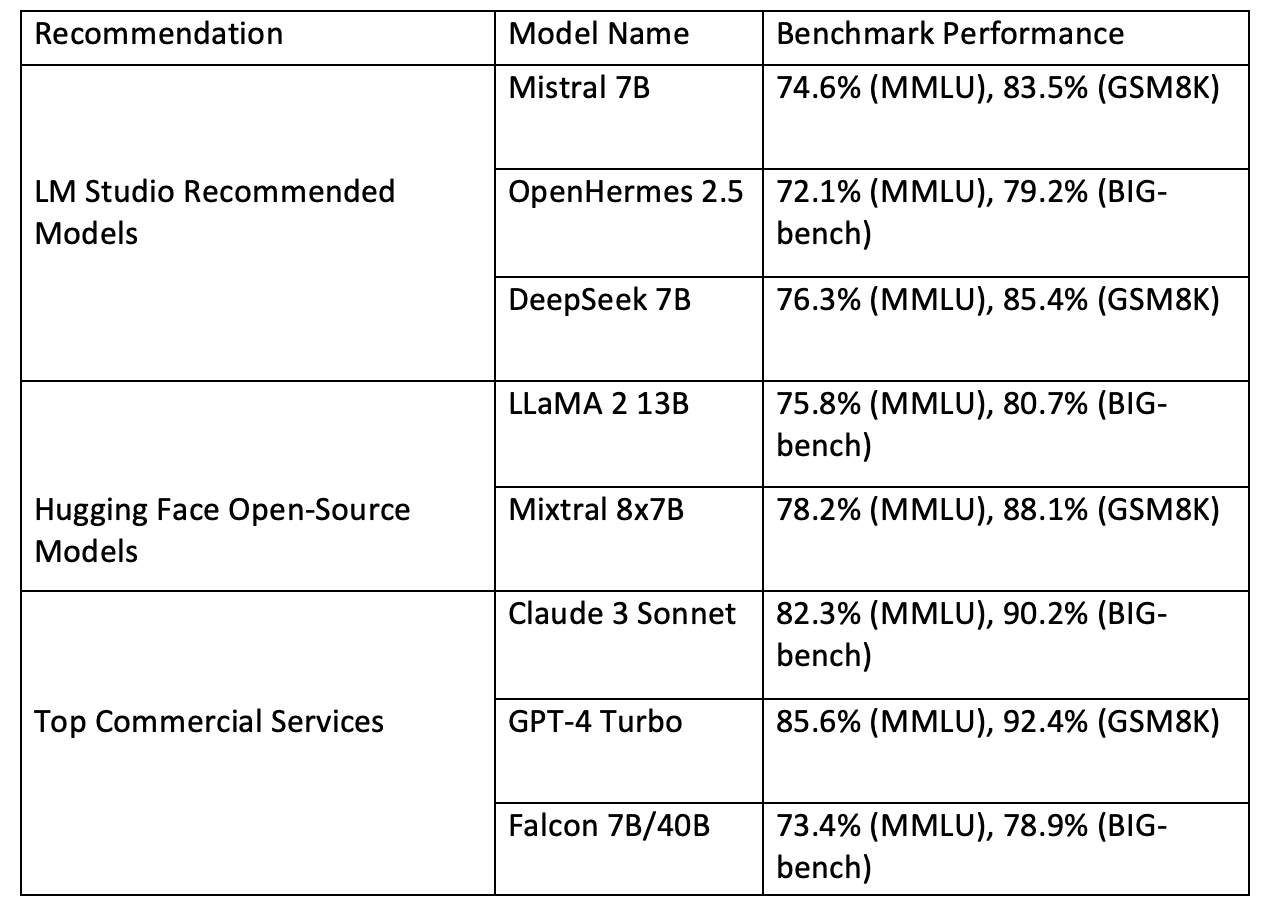
\includegraphics[width=\linewidth]{Fig/Selected_LLM.png}
    \caption{Selected Models for Experimentation}
    \label{fig:enter-label}
\end{figure}

% \textbf { Can LLMs effectively enhance decision making for AVs in Unknown-Unsafe domains within a multi-agent framework compared to current mechanisms?}
Hugging Face\footnote{https://huggingface.co/}is a platform where various open LLM models are available. LM Studio\footnote{https://lmstudio.ai/} is a platform to test and integrate LLM available on Hugging Face a locally available system on ordinary computing devices, even without powerful GPUs. Now, the question is what factors were considered in the selection of LLMs for this study? One key factor in our model selection was quantization, which optimizes model performance while reducing computational requirements. This research \cite{Jin2024ACE} indicates that 8-bit quantization enables the majority of LLMs to maintain a performance level comparable to their nonquantized equivalents, regardless of model size (e.g. 7B to 70B parameters). Moreover, LLMs that are quantized to 4 bits can also up hold similar performance to their non-quantized versions across most benchmarks. This approach achieves memory reduction of 50 to 75 \% while preserving precision in complex tasks such as reasoning, decision making, and domain-specific applications. 
The models chosen for this investigation were selected using a structured approach based on three key factors: popularity and performance in text-to-text generation, LM Studio recommendations for optimized accuracy, and comparative evaluations of the top commercial services. Specifically, 1) Some models were chosen based on the highest number of downloads from Hugging Face, ensuring widespread adoption and benchmark effectiveness. 2) Models suggested by LM Studio were included due to their strong performance and compatibility with local inference environments. 3) The best commercial services were selected based on their comparative performance with open-source counterparts, prioritizing accuracy, interpret ability, and real-time inference. The selected models are shown in Fig. 3. However, not all Hugging Face models are fully compatible with the LM Studio runtime. As a result, some models were tested directly on the Hugging Face interface to avoid compatibility issues. Furthermore, while models such as OpenAI’s o1, DeepSeek R1, and Llama 3.1 405B have demonstrated strong benchmark performance, they were not included in this study due to limited quantization support, lack of local deployment feasibility, and restricted open-source availability.
To test these selected models model, we will prepare simple text-based scenarios. Some of these scenarios will involve situations that can only be solved through logical reasoning, while others will require recognizing and applying common or well-known information (e.g. stopping when seeing a red traffic light). These scenarios will be used as input for various LLMs to assess how effectively they handle both types of challenges. The experiments will be conducted using the LLM selected in Fig.4. The purpose was to assess whether the models could accurately recommend actions based on the complexity and ambiguity of each scenario.  A major consideration was consistency. \textbf{Does repeated querying of LLMs on the same scenario lead to variations in decision-making outcomes?} To test this, we posed each scenario to each model at least 20 times. This helped us to check whether the models could provide stable and repeatable outputs or whether their decisions varied. This consistency is crucial for tasks like AV decision-making, where unpredictable output could lead to safety risks.


% The chosen models are shown in Fig. 4. One thing to note is that not all the models available on Hugging Face are compatible with the LM Studio runtime. Therefore, we ran some of the chosen models from Hugging Face on the Hugging Face interface itself due to compatibility issues.The models used for this investigation are selected in three ways: 1. Some text-to-text generation models have been chosen based on the highest number of downloads from Hugging Face, 2. The models suggested by LM Studio are considered as they offer best performance and accuracy, 3. The top commercial services that are openly available are taken into account on the basis of the performance evaluation with other commercial services. The chosen models are shown in Fig. 4. One thing to note is that not all the models available on Hugging Face are compatible with the LM Studio runtime. Therefore, we ran some of the chosen models from Hugging Face on the Hugging Face interface itself due to compatibility issues.


% For each scenario, we asked the same question to each language model at least 20 times. The purpose was to check whether the model could give the same answer every time or if its decision would change. This helps us understand how consistent and reliable the models are when used in critical tasks like deciding whether an autonomous vehicle should "STOP" or "FORWARD" in difficult situations.


% In our research, we will create specific scenarios and use them as inputs for LLM to see if they can demonstrate human-like reasoning in unknown unsafe situations. By examining how well LLMs can handle these scenarios, our objective is to determine whether they can improve the current struggles faced by AVs.
% We will run this test on various cloud base and local base LLM.

% To address this, we will design various custom scenarios requiring logical reasoning or common knowledge (e.g., stopping at a red light) and use them as inputs to different LLMs. By evaluating how well these models navigate such situations, we aim to assess their potential to overcome the challenges faced by current AV systems. These experiments will be conducted using cloud-based and locally deployed LLMs.


% Now lets introduce the output from different LLM and disscuss about the input and also i gonna disscuss about the assumption.

\begin{figure}[h]
    \centering
    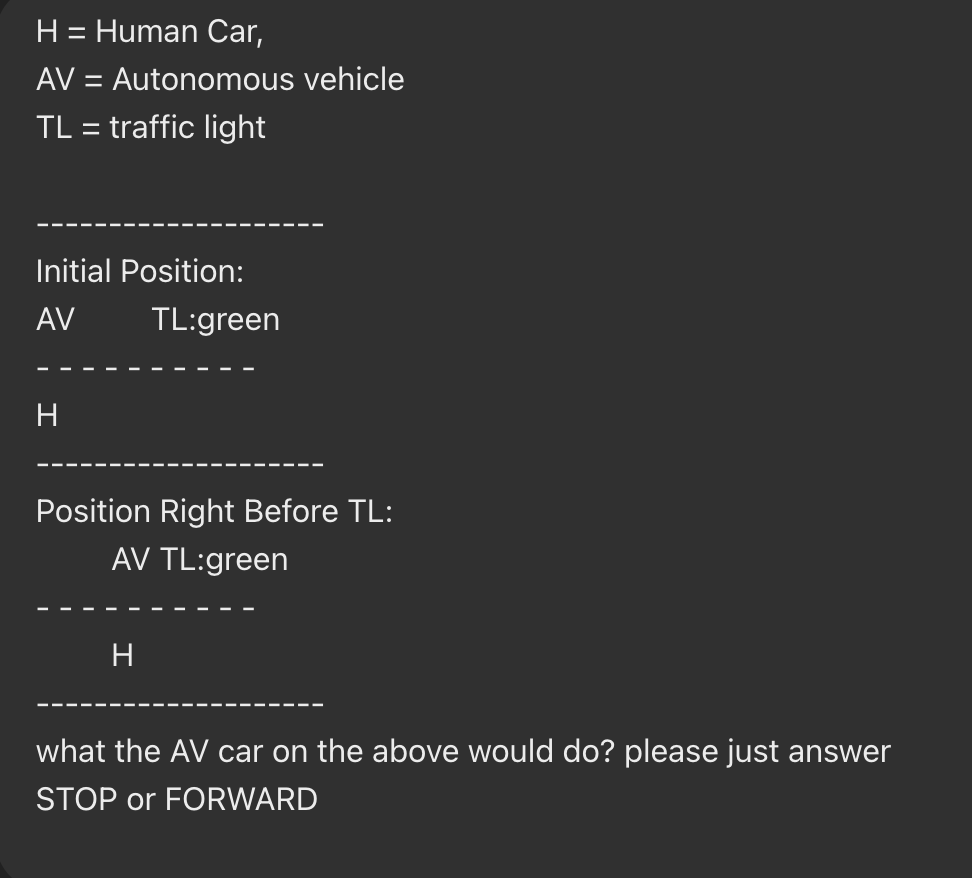
\includegraphics[width= \linewidth]{Scenario.png}
    \caption{Text-base scenario}
    \label{fig:enter-label}
\end{figure}



% Several scenarios representing both "known-safe" and "unknown-unsafe" situations, where decision-making may be straightforward or ambiguous for autonomous vehicles, were presented to various language models. These scenarios were converted into text-based natural language prompts to simulate real-world decision-making challenges. For consistency, we added the instruction: "What should the AV do in the above situation? Please, just answer with 'STOP' or 'FORWARD'." 

% For each test scenario, we have queried each model at least 20 times to assess consistency and determine whether the model could reliably produce the same result in multiple runs.
\begin{figure}[h]
     \centering
     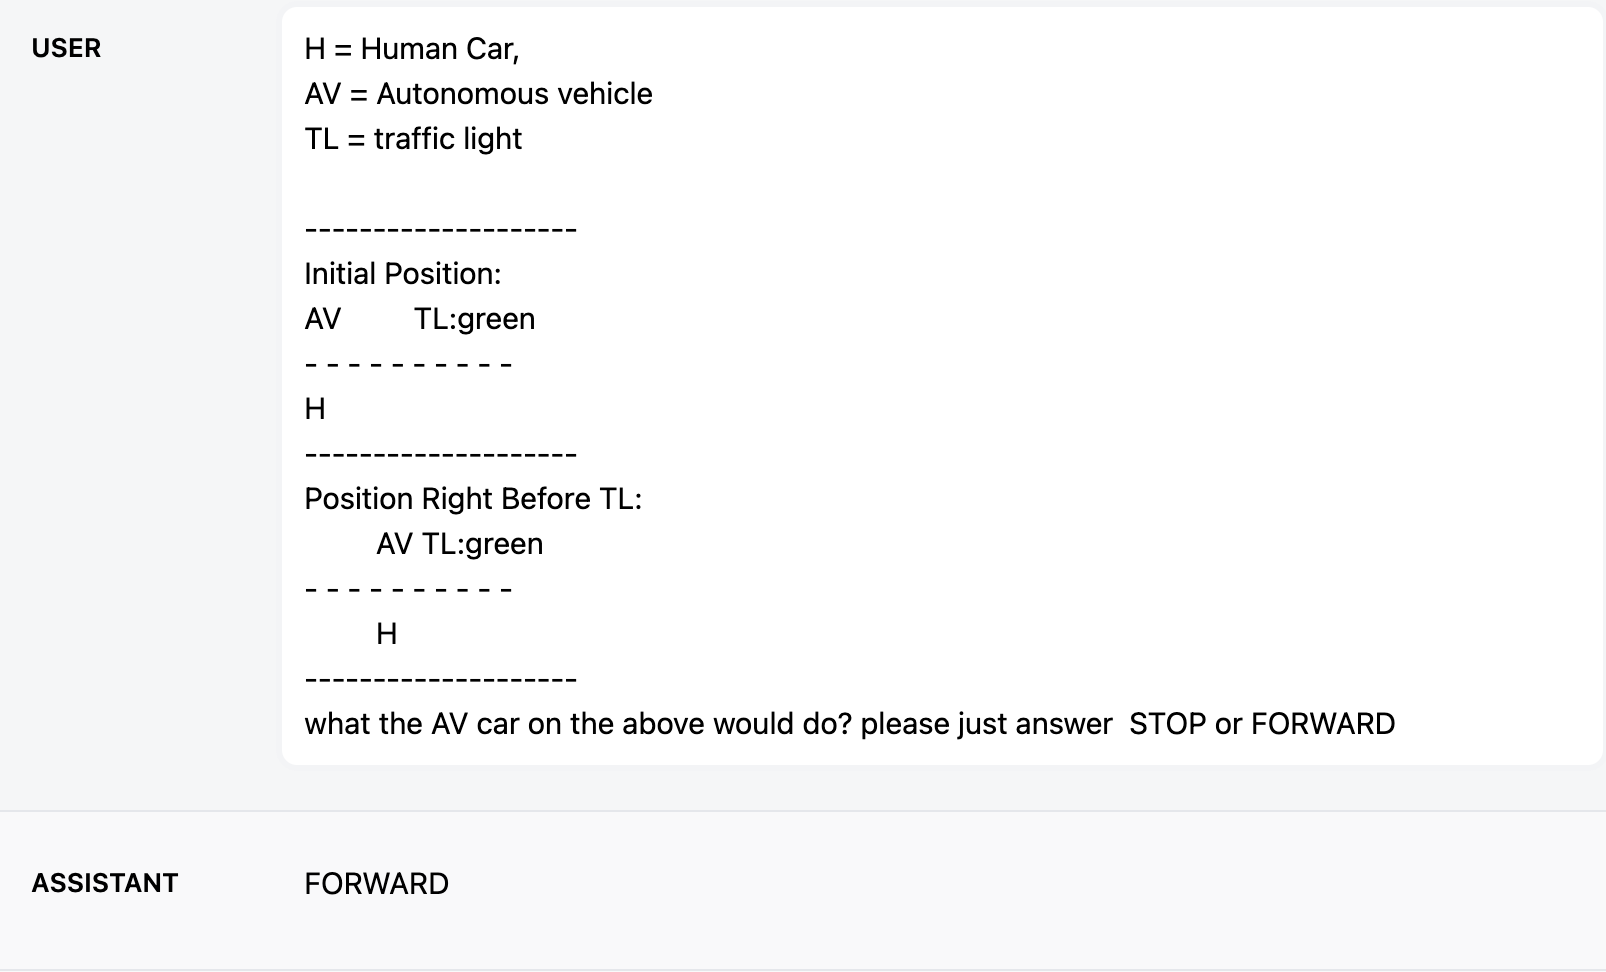
\includegraphics[width= \linewidth]{Fig/FROM_LLM.png}
     \caption{LLM Model Response}
     \label{fig:enter-label}
 \end{figure}
We presented a text-based scenario showing the autonomous vehicle (AV) and human-driven car (H) approaching a green traffic light similar to the one in Fig. 4, to the language models. We used the following prompt: What would the AV do in this situation? Please, just answer STOP or FORWARD. We ran this same prompt at least 20 times in OpenHermes-2.5-Mistral-7B and analyzed the results.

 % \begin{figure}[h]
 %     \centering
 %     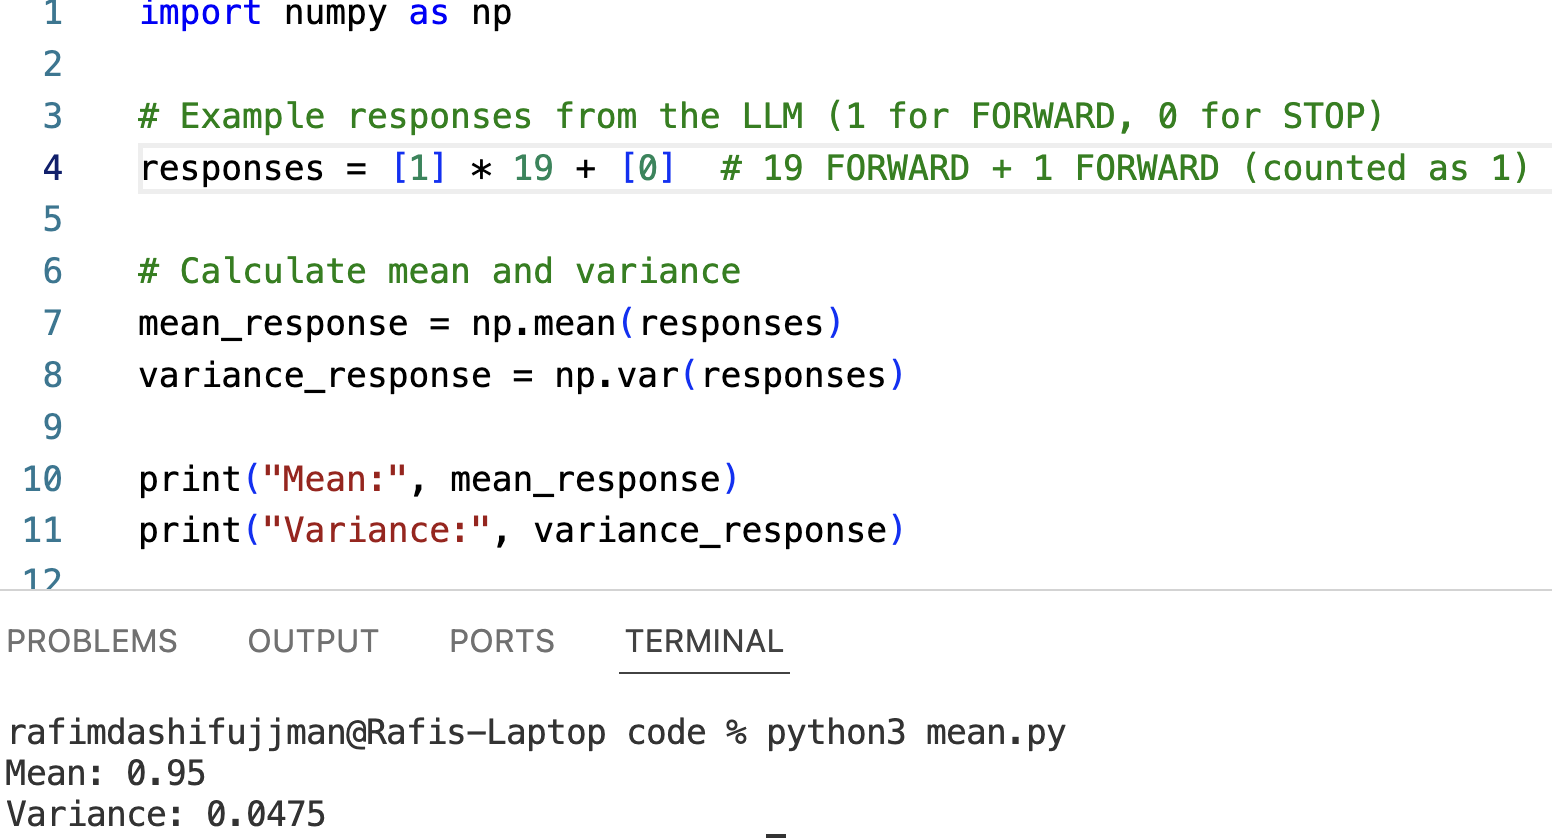
\includegraphics[width=\linewidth]{Fig/mean.png}
 %     \caption{LLM Model Response Analysis}
 %     \label{fig:enter-label}
 % \end{figure}
 
 \begin{figure}[h]
     \centering
     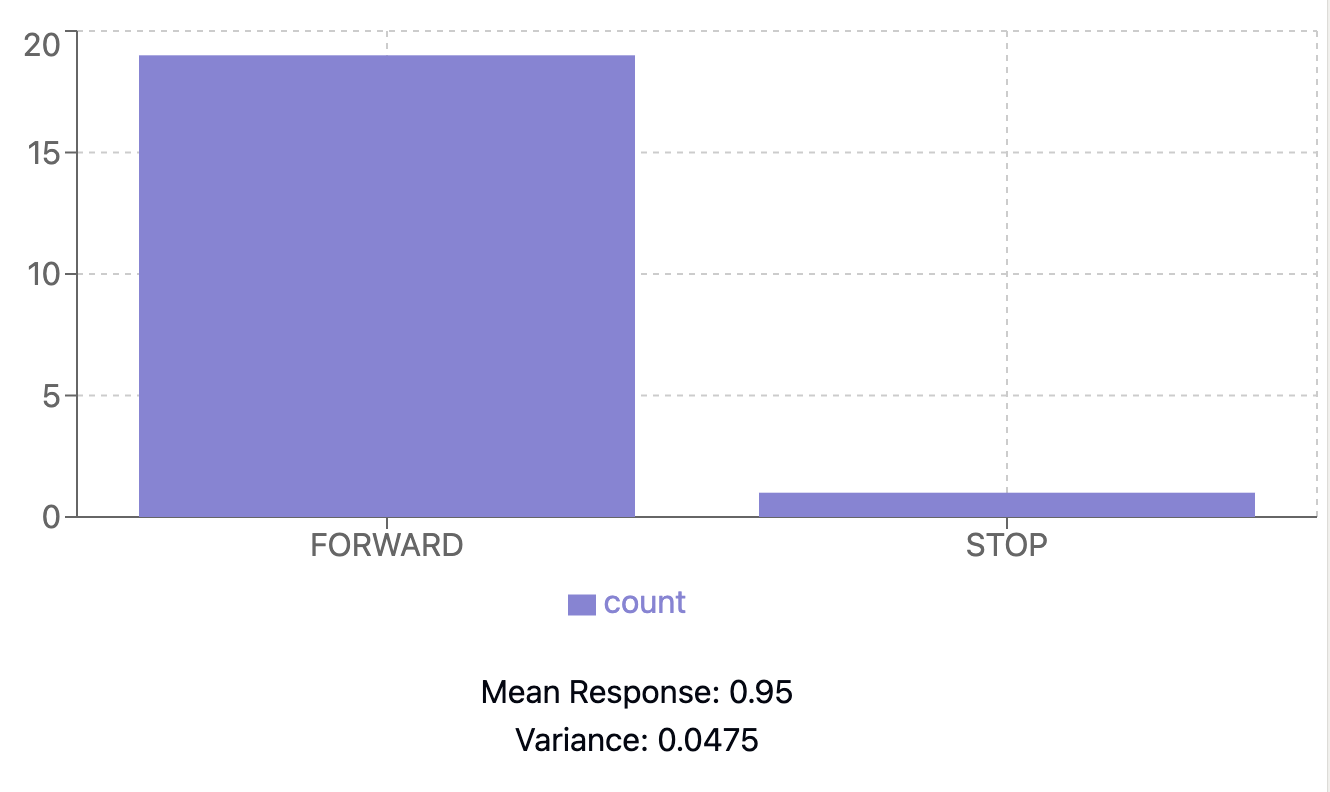
\includegraphics[width=\linewidth]{Fig/chart.png}
     \caption{LLM Model Response Analysis}
     \label{fig:enter-label}
 \end{figure}
 


\begin{figure*}[h]
    \centering
    % First Row
    \begin{subfigure}[b]{0.3\textwidth}
        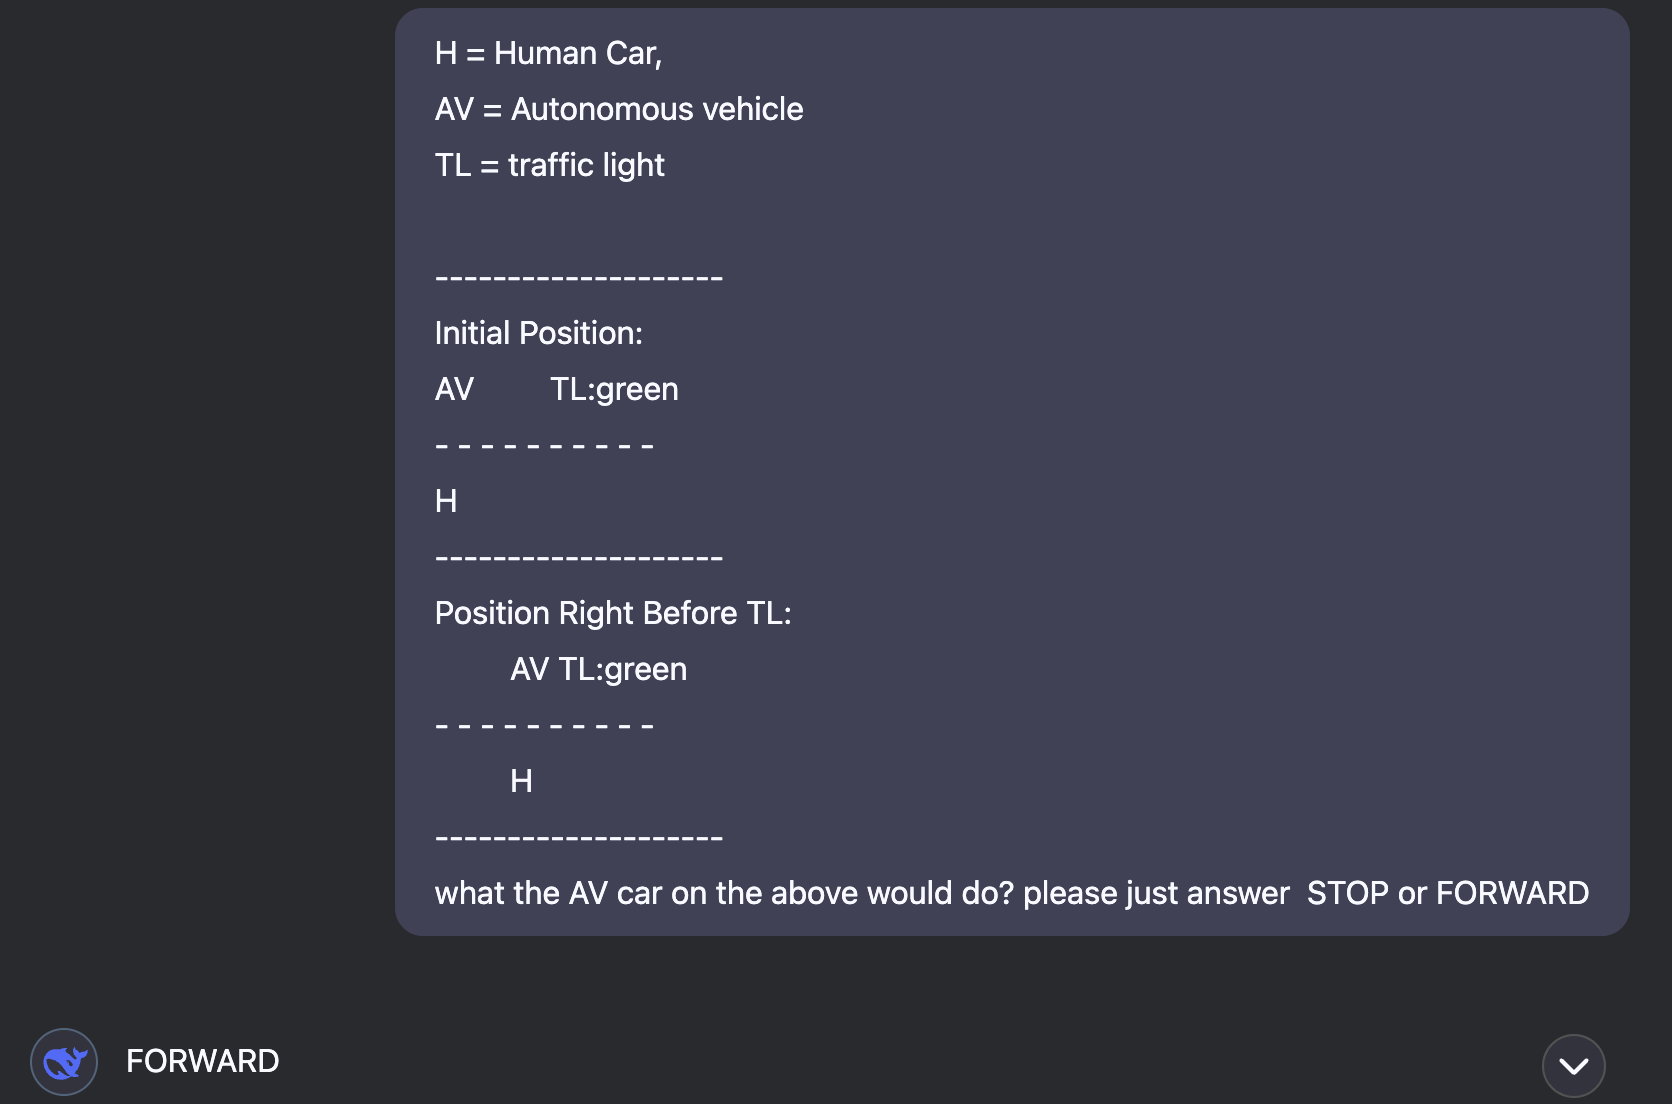
\includegraphics[width=\linewidth]{outfromLLM/deepq_TL.png}
        \caption{Output from DeepQ}
    \end{subfigure}
    \hfill
    \begin{subfigure}[b]{0.3\textwidth}
        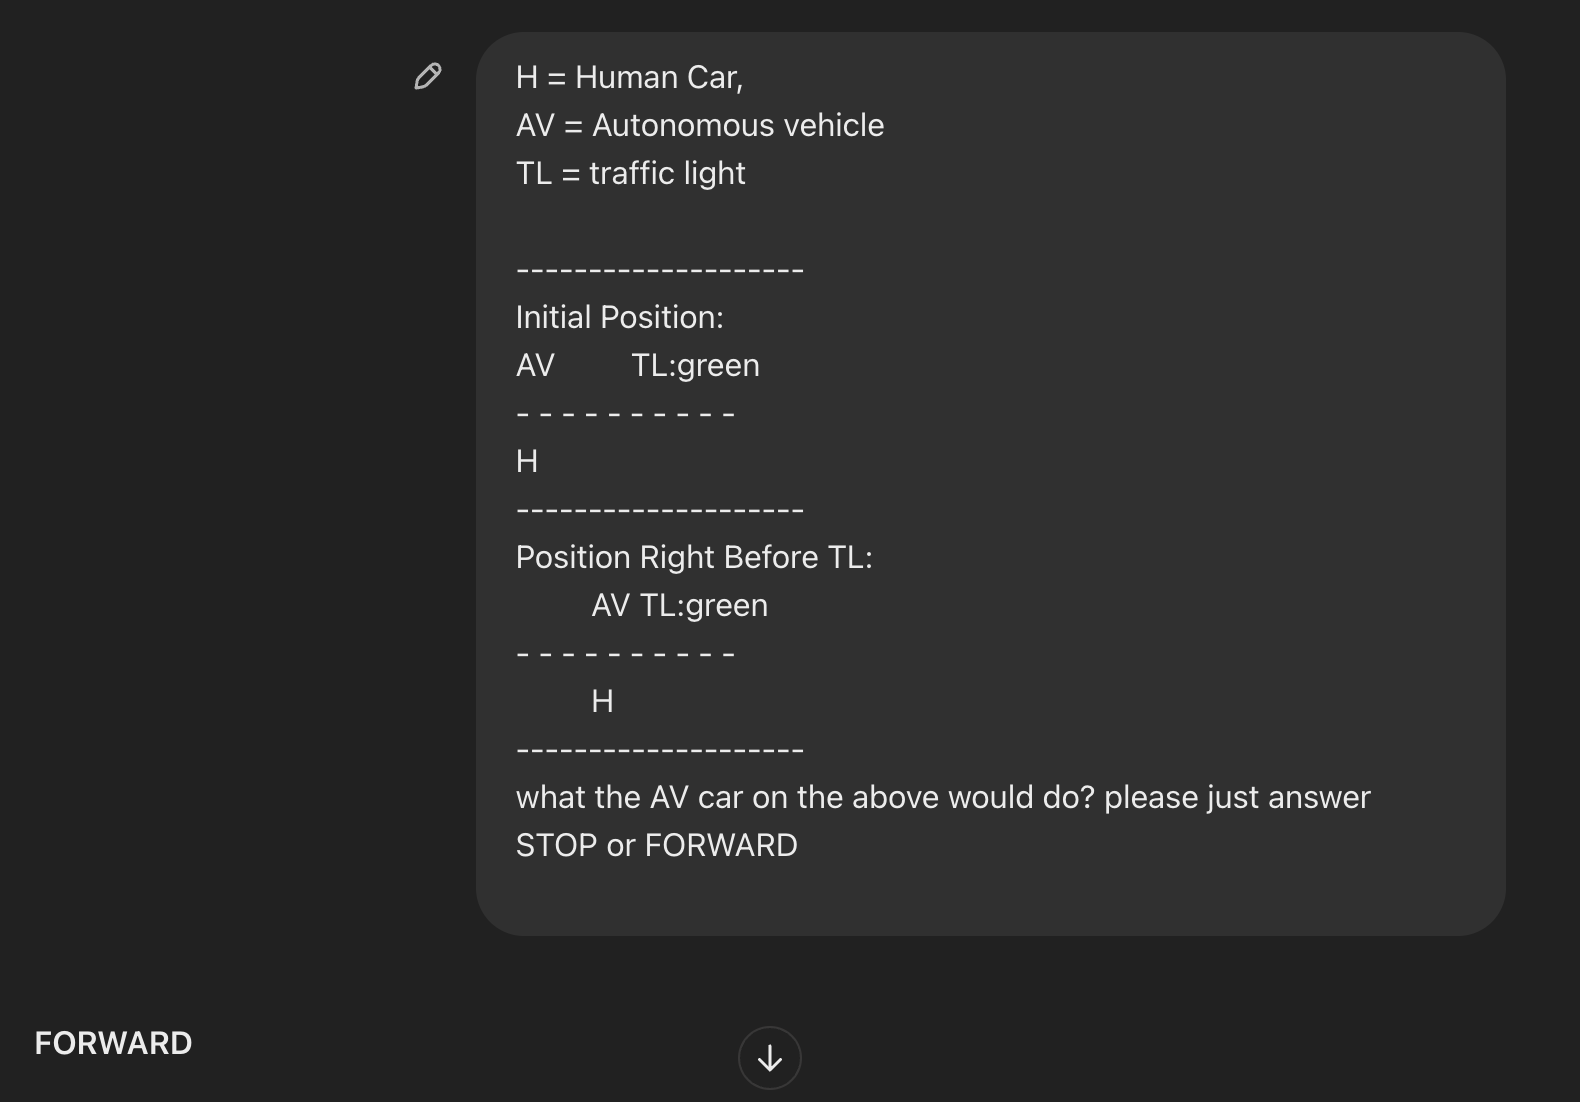
\includegraphics[width=\linewidth]{outfromLLM/GPT_TL.png}
        \caption{Output from ChatGPT}
    \end{subfigure}
    \hfill
    \begin{subfigure}[b]{0.3\textwidth}
        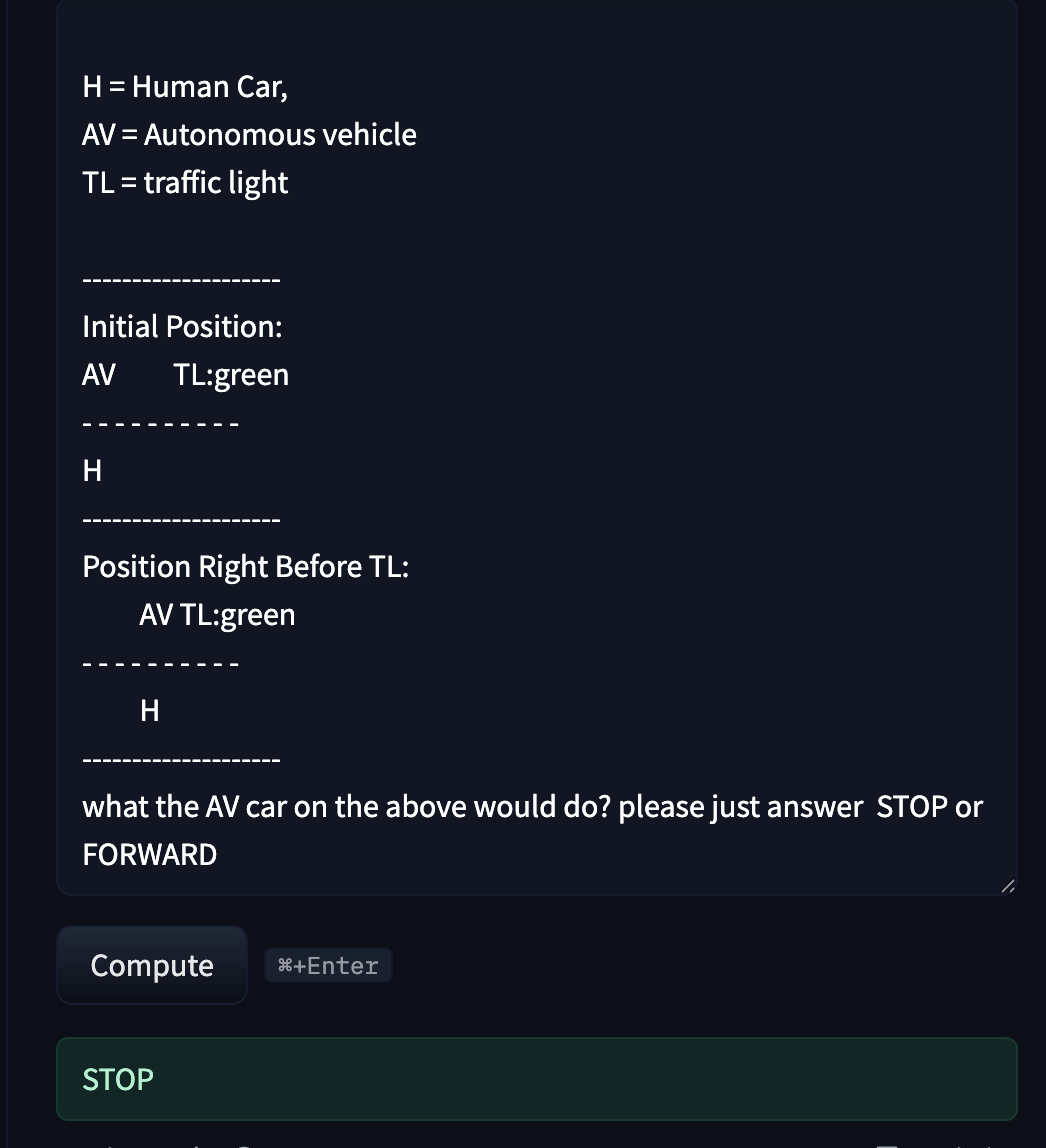
\includegraphics[width=\linewidth]{outfromLLM/google:flan-t5-large.png}
        \caption{Output from google/flan-t5-large}
    \end{subfigure}

    % Space between rows
    \vspace{1em}

    % Second Row
    \begin{subfigure}[b]{0.3\textwidth}
        \includegraphics[width=\linewidth]{outfromLLM/claude.png}
        \caption{Output from Claude}
    \end{subfigure}

    \caption{Comparison of responses from different LLMs on the task}
    \label{fig:llm_outputs}
\end{figure*}





% this is the reference part
\bibliographystyle{ieeetr}
\bibliography{references}
\end{document}


